\section{Referencia de la Clase List\-Comp\-Articulo}
\label{classListCompArticulo}\index{ListCompArticulo@{ListCompArticulo}}
Administra el listado de componentes de un art\'{\i}culo.  


{\tt \#include $<$comparticulolist.h$>$}

Diagrama de colaboraci\'{o}n para List\-Comp\-Articulo:\begin{figure}[H]
\begin{center}
\leavevmode
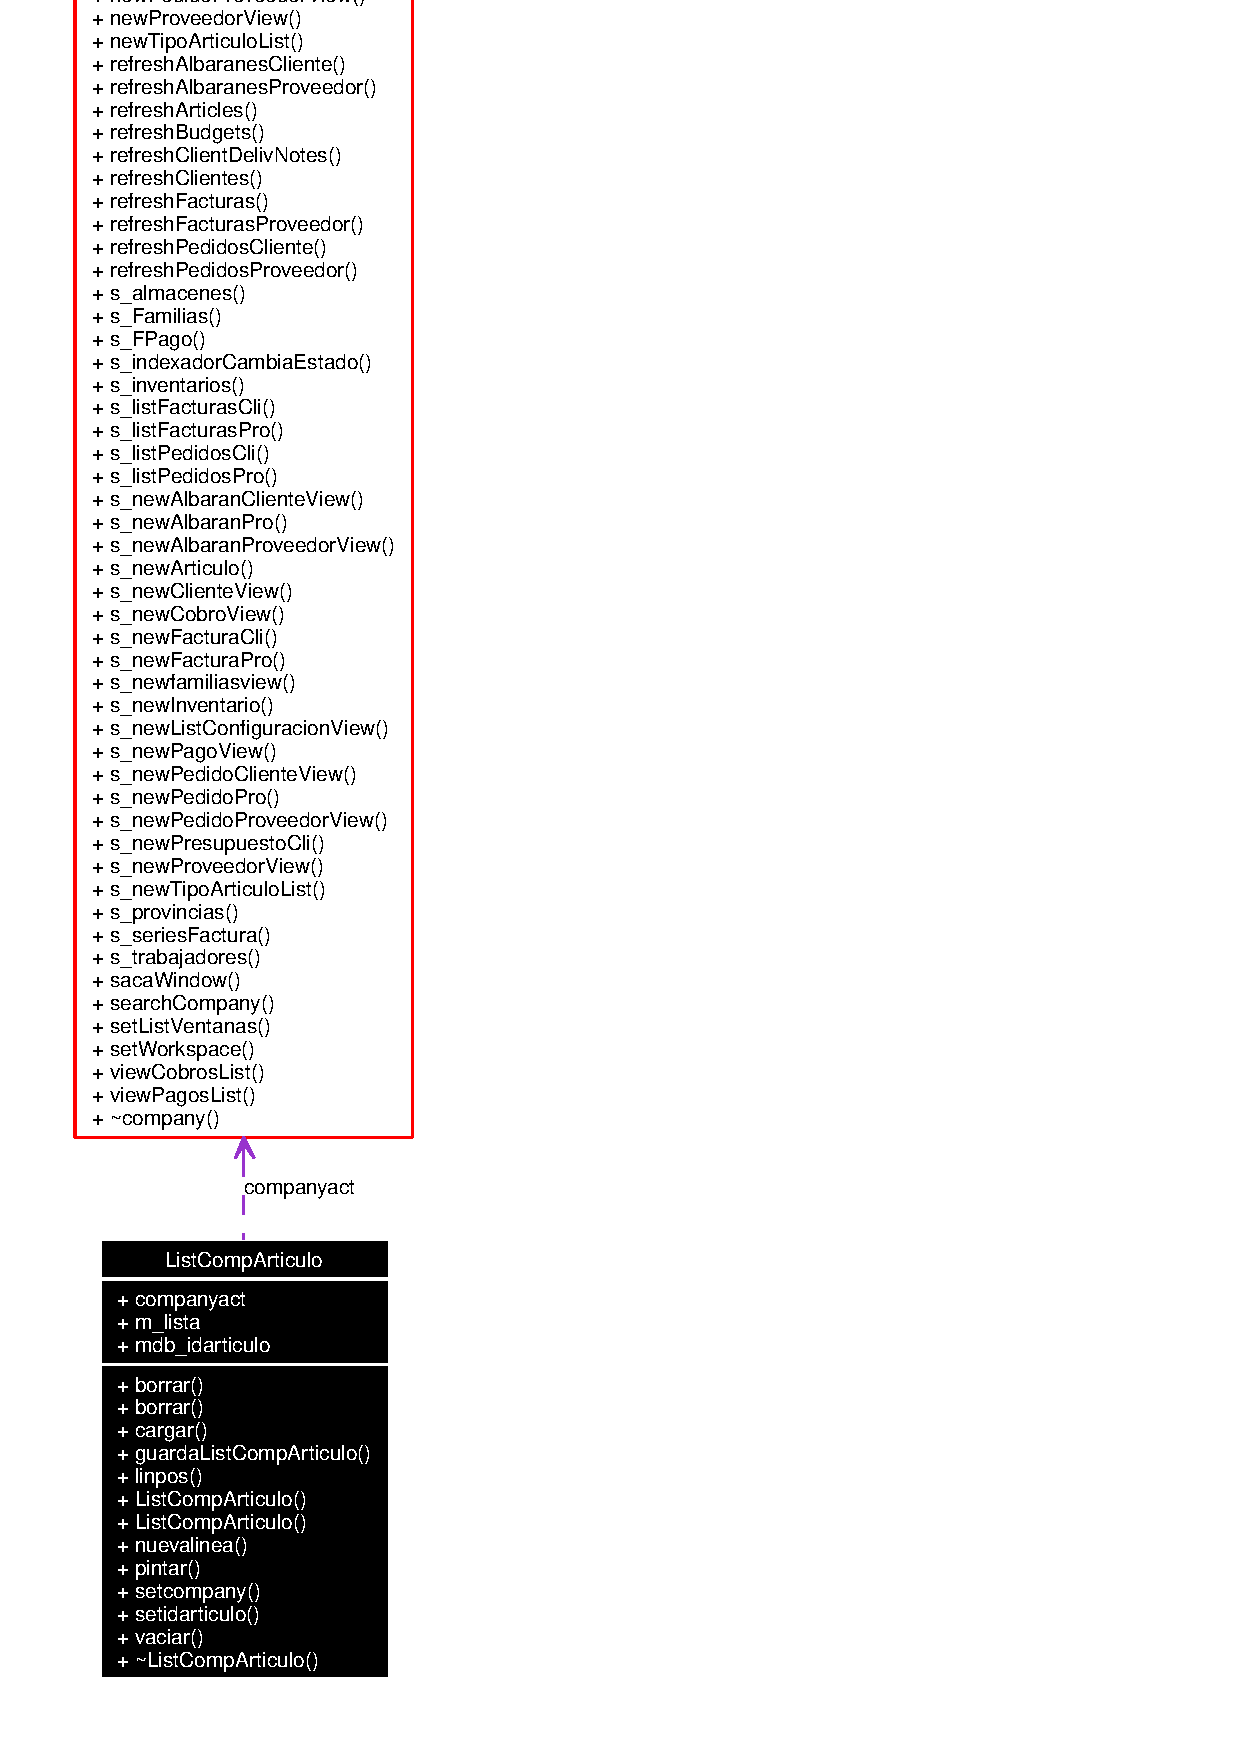
\includegraphics[width=99pt]{classListCompArticulo__coll__graph}
\end{center}
\end{figure}
\subsection*{M\'{e}todos p\'{u}blicos}
\begin{CompactItemize}
\item 
void {\bf borrar} (int)\label{classListCompArticulo_a0}

\item 
void {\bf borrar} ()\label{classListCompArticulo_a1}

\item 
void {\bf cargar} (QString)
\begin{CompactList}\small\item\em Carga lineas de presupuesto. \item\end{CompactList}\item 
void {\bf guarda\-List\-Comp\-Articulo} ()\label{classListCompArticulo_a3}

\item 
{\bf Comp\-Articulo} $\ast$ {\bf linpos} (int)\label{classListCompArticulo_a4}

\item 
{\bf List\-Comp\-Articulo} ({\bf company} $\ast$comp)\label{classListCompArticulo_a6}

\item 
void {\bf nuevalinea} (QString, QString, QString, QString)\label{classListCompArticulo_a7}

\item 
virtual void {\bf pintar} ()\label{classListCompArticulo_a8}

\item 
void {\bf setcompany} ({\bf company} $\ast$c)\label{classListCompArticulo_a9}

\item 
void {\bf setidarticulo} (QString id)\label{classListCompArticulo_a10}

\item 
void {\bf vaciar} ()\label{classListCompArticulo_a11}

\end{CompactItemize}
\subsection*{Atributos p\'{u}blicos}
\begin{CompactItemize}
\item 
{\bf company} $\ast$ {\bf companyact}\label{classListCompArticulo_o0}

\item 
QList$<$ {\bf Comp\-Articulo} $\ast$ $>$ {\bf m\_\-lista}\label{classListCompArticulo_o1}

\item 
QString {\bf mdb\_\-idarticulo}\label{classListCompArticulo_o2}

\end{CompactItemize}


\subsection{Descripci\'{o}n detallada}
Administra el listado de componentes de un art\'{\i}culo. 



\subsection{Documentaci\'{o}n de las funciones miembro}
\index{ListCompArticulo@{List\-Comp\-Articulo}!cargar@{cargar}}
\index{cargar@{cargar}!ListCompArticulo@{List\-Comp\-Articulo}}
\subsubsection{\setlength{\rightskip}{0pt plus 5cm}void List\-Comp\-Articulo::cargar (QString {\em idarticulo})}\label{classListCompArticulo_a2}


Carga lineas de presupuesto. 

Creamos un elemento del tipo {\bf Comp\-Articulo}{\rm (p.\,\pageref{classCompArticulo})} y lo agregamos a la lista. 

La documentaci\'{o}n para esta clase fu\'{e} generada a partir de los siguientes archivos:\begin{CompactItemize}
\item 
comparticulolist.h\item 
comparticulolist.cpp\end{CompactItemize}
